\documentclass[12pt]{article}
\usepackage{achemso}
\usepackage[margin=1.0in]{geometry}
\usepackage{setspace}
\usepackage{amsmath}             % for equation typesetting
\usepackage{amssymb}             % for equation typesetting
\usepackage{mathrsfs} 
\usepackage{wasysym}             % for geometric shapes
\usepackage{color}               % for colored fonts
\usepackage{setspace}            % for 1.5 and double spacing
\usepackage{graphicx}            % main graphics package
\usepackage{wrapfig}             % allow text wrapping around figures
\usepackage{subcaption}
\usepackage{multirow}
%\doublespacing

\usepackage{appendix}

\usepackage[capitalize]{cleveref}
\crefname{figure}{Fig.}{Figs.}
\Crefname{figure}{Figure}{Figures}
\crefname{table}{Tab.}{Tabs.}
\Crefname{table}{Table}{Tables}
\crefname{equation}{Eq.}{Eqs.}
\Crefname{equation}{Equation}{Equations}
\crefname{section}{Sec.}{Secs.}
\Crefname{section}{Section}{Sections}
\crefname{appsec}{appendix}{appendices}
\Crefname{appsec}{Appendix}{Appendixes}

%\usepackage{titlesec}
%\titleformat*{\section}{\Large\bfseries}
%\titleformat*{\subsection}{\large\bfseries}

% Mathematical Shortcuts
\newcommand{\pfrac}[2]{\frac{\partial #1}{\partial #2}}   % partial derivative
\newcommand{\difrac}[2]{\frac{d #1}{d #2}}                % derivative
\newcommand{\bpar}[1]{\left( #1 \right)}                  % big parentheses
\newcommand{\bbra}[1]{\left[ #1 \right]}                  % big brackets
\newcommand{\bbar}[1]{\left| #1 \right|}                  % big bars
\newcommand{\bra}[1]{\left\langle #1 \right\vert}         % bra
\newcommand{\ket}[1]{\left\vert #1 \right\rangle}         % ket
\newcommand{\inner}[2]{\left\langle #1 \left\vert\right. #2 \right\rangle}            % bracket
\newcommand{\innerop}[3]{\left\langle #1 \left\vert #2 \right\vert #3 \right\rangle}  % operator matrix element
\newcommand{\innersub}[4]{\langle \bd{#1}_{#2}, \bd{#3}_{#4} \rangle}                 % bracket with subscripts
\newcommand{\half}{\frac{1}{2}}                           % 1/2
\newcommand{\powfrac}[3]{\bpar{\frac{#1}{#2}}^{#3}}       % fraction raised to a power
\newcommand{\ii}{\infty}                                  % infinity symbol
\newcommand{\tquad}{\quad\quad\quad}                      % triple-quad spacing
\renewcommand{\Im}{\text{Im}}                             % imaginary symbol
\renewcommand{\Re}{\text{Re}}                             % real symbol

\newcommand*\mycommand[1]{\texttt{\emph{#1}}}
\newcommand*\suchthat[0]{\text{ }\vert\text{ }}
\newcommand*\complexmatfield[1]{\mathbb{C}^{#1\text{x}#1}}
\newcommand*\speciallinear[2]{\mathrm{UnL}(#1,#2)}
\newcommand*\complexspeciallinear[1]{\speciallinear{#1}{\mathbb{C}}}
\newcommand*\generallinear[2]{\mathrm{GL}(#1,#2)}
\newcommand*\complexgenerallinear[1]{\generallinear{#1}{\mathbb{C}}}
\newcommand*\mat[1]{\boldsymbol{#1}}

\newcommand*\vc[1]{\boldsymbol{#1}}
\newcommand*\op[1]{\mathcal{#1}}

\newcommand*\mylinesp[0]{\linespread{1.489}}
\mylinesp

\title{General Exam}
\date{October 19, 2016 \\ CHB 239}
\author{David Williams-Young\\ Department of Chemistry, University of Washington}


\begin{document}
\linespread{1.0}
\maketitle
\mylinesp
\newpage
\section{Introduction}

Formally spin--forbidden processes, such as intersystem crossing (ISC),  play an
crucial role in photochemistry.\cite{Marian_SOC,Scaiano_Photo,Steer93_CR67} ISC
is a transition between quantum states of differing spin multiplicity which
manifests either radiatively or non-radiatively.  The functionality of many
modern technologies, such as phosphorescent organic light emitting diodes
(PHOLEDs)\cite{Miyaguchi99_JAP1502}, depend heavily on finely tuned ISC to
control the rate of population and depopulation of triplet intermediate states
from singlet states upon photoexcitation. The fact that the non--relativistic
treatment of molecular quantum mechanics predicts phenomena such as ISC as
formally forbidden, it has been long thought that the time--scales at which
they occur are far too long to compete with transitions between states of the
same spin multiplicity.\cite{Marian_SOC} However, recent studies have shown
that this is not necessarily the case, and that ISC can indeed be competitive
even at short time--scales.\cite{Marian_SOC,Li16_JA2,Lim74_CPL}  ISC is an
inherently relativistic, and non--adiabatic time--dependent
process\cite{Dyall07_book,Reiher15_book}.  Thus to accurately treat these
phenomena theoretically, one must provide an \emph{ab initio} description of
the relativistic effects throughout the non--adiabatic time--evolution of the
quantum system.  {\bf While much effort has been directed at the accurate
treatment of non--adiabatic molecular dynamics, the scope of inquiry has been
primary limited to non--relativistic regime.}

Relativistic effects, while often neglected in most standard treatments of
quantum mechanics, can have profound consequences in chemical
systems.\cite{Pyykko12_45} Scalar relativistic effects cause the contraction of
the core electron shells of heavy atoms, but perhaps of even more consequence is
the introduction of spin couplings in the Hamiltonian.  Spin-spin (SSC) and
spin-orbit (SOC) coupling can affect the electronic spin dynamics even in light
atoms. 
%A direct consequence of these couplings on the electronic manifold is the
%breaking of spin--symmetry as the Hamiltonian no longer commutes with the spin
%operator, $\op{S}$. 
This introduction of spin--couplings is what allows, at an
operator level, for formally spin--forbidden processes to occur, namely
ISC. 
%Although some approaches have been purposed to account for SOC in the
%treatment of the electronic manifold perturbatively\cite{Thiel14_JCP124101},
%these approximations will break down whenever SOC is non--negligible. 
%Further,
%these treatments neglect any contributions from many--body SOC or SSC, which
%must be present for a proper treatment of spin interaction. 
%Hence a
%relativistic, variational, and well balanced approach much be adopted to account
%for these interactions for the general case. 
There exist several \emph{ab
initio} methods to approximately treat these relativistic effects, however, in
this work the discussion will be limited to two--component relativistic
Hamiltonians, specifically the ``exact two--component" (X2C) Hamiltonian.
\cite{Liu05_241102,Peng06_044102,Saue07_064102,Peng09_031104,Reiher13_184105,Cheng07_104106,Liu16_204}
This choice of two--component transformation is due to its simplicity and
accuracy.  A brief overview of the X2C method may be found in \cref{sec:X2C}.

In the quantum mechanical description of molecular systems, time evolution of
the total molecular wave function, $\ket{\Psi (t)}$ is governed by the
Hamiltonian wave equation (in atomic units),
\begin{equation}
\op{H}(t) \ket{\Psi (t)} = i\partial_t \ket{\Psi(t)} \quad,
\label{eq:WaveEq}
\end{equation}
where $\op{H}(t)$ is the time--dependent Hamiltonian, $\partial_t$ is a partial
derivative with respect to time, and $t$ is a time parameter.  In principle, one
may solve \cref{eq:WaveEq} (in some approximate manner) simultaneously for both
the electronic and nuclear degrees of freedom explicitly. However, this approach
is  intractable for quantum systems exceeding more than a few particles. To
simplify the time integration of \cref{eq:WaveEq}, one may formally decompose
$\ket{\Psi (t)}$ into a product of nuclear and electronic wave functions,
\begin{equation} 
\ket{\Psi (t)} = \ket{\Phi(\vc{R}(t),t)}\otimes\ket{\Theta(t)} 
\quad .  
\label{eq:exactSepElecNuc}
\end{equation} 
Here, $\ket{\Phi(\vc{R}(t),t)}$ and $\ket{\Theta (t)}$ are the electronic and
nuclear wave functions respectively and $\vc{R}(t)$ is the expectation value of
the nuclear position operator, $\vc{R}(t) =
\innerop{\Theta(t)}{\hat{\vc{R}}}{\Theta(t)}$.  
This formally exact treatment\cite{Gross10_PRL123002, Cederbaum08_JCP124101,
Ghosh15_MP1} allows one to, at least in in principle, bifurcate the treatment of
quantum molecular dynamics into explicit treatment of the electronic and nuclear
time dependence separately.  

When obtaining the time evolution of the total molecular wave function, it is
often advantageous to work in so called adiabatic basis of quantum states,
\begin{equation}
\op{H}(t) \ket{\Psi_I (t)} = E_I(t) \ket{\Psi_I (t)}
\quad \forall t, I \in \mathbb{N},
\label{eq:EigSpec}
\end{equation}
where $\ket{\Psi_I}$ and $E_I$ represent the $I$-th adiabatic wave function and
eigenenergie, respectively.  Taking the separation of the total wave function in
\cref{eq:exactSepElecNuc}, we may rewrite the total wave function as a linear
combination of adiabatic states,
\begin{equation}
\ket{\Psi (t)} = c_I \ket{\Phi_I (\vc{R}(t),t)} \otimes \ket{\Theta_I (t)}
\quad ,
\label{eq:AdiaExp}
\end{equation}
where $\{ c_I \}$ is a set of expansion coefficients, and $\{\ket{\Phi_I}\}$ and
$\{\ket{\Theta_I}\}$ are the sets of electronic and nuclear adiabatic wave
functions, respectively. Given a complete eigenspectrum of \cref{eq:EigSpec},
the expansion in \cref{eq:AdiaExp} is formally exact, thus the problem now
becomes how to properly obtain the adiabatic electronic and nuclear wave
functions.

Over the years, perhaps the most successful \emph{ab initio} treatment of the
adiabatic electronic wave function has been in the configuration interaction
(CI) expansion of the electronic wave function.
\cite{Meyer00_PR1,Knowles88_JCP1,Handy82_JCP1,Saalfrank04_JCP124102,
Schlegel92_CPL524,Handy84_CPL315,Joergensen78_JCP3833,Fleig08_JCP014108}
A brief overview of the CI method may be found in \cref{sec:ci}.  Many
successful attempts have been made to extend CI variants to relativistic
Hamiltonians\cite{Neese13_JCP104113, Olsen97_TCA125, Jensen96_JCP4083,
Fleig08_JCP014108}, including my recent work on the extension of the
particle--particle Tamm-Dancoff approximation (pp-TDA) to the X2C method
\cite{DBWY16_Accepted1} of which results are presented in \cref{sec:pp-X2C}. The
CI method is simplest method, in formalism, for the addition of explicit
many--body interaction back into mean--field description of the ground state
electronic wave function such as Hartree--Fock. In addition to correcting the
uncorrelated behavior of mean--field ground states, the CI method is also able
to treat excited electronic states in a correlated manner, making it a suitable
method for use in non--adiabatic molecular dynamics.

There exist a vast plethora of computational methods to treat non--adiabatic
molecular dynamics based on the separation in
\cref{eq:exactSepElecNuc,eq:AdiaExp}.
\cite{Meyer00_PR1,Li11_144102,Li05_084106,Preston71_562}
For the purposes of this work, the discussion will be restricted to that of the
trajectory surface hopping (TSH) method.  TSH is one of the most widely applied
methods for simulating electronically non-adiabatic dynamics of molecular and
condensed-phase systems.\cite{Barbatti11_1759, Tavernelli14_62, Tully12_22A301,
Tully98_407, Hynes14_97} At its core, TSH is a stochastic algorithm that
controls which electronic adiabat dictates the forces on the nuclei during a
classical nuclear trajectory.\cite{Preston71_562} As a semi-classical method,
the time--evolution of the electronic degrees of freedom are treated as quantum
mechanical while the time evolution of the nuclear positions are treated as
classical through Newton's equations of motion. 
%In essence, this classical treatment may be
%thought of as the nuclear wave function begin written as a product of delta
%functions centered at the classical nuclear positions
%\begin{equation}
%\inner{\vc{R}}{\Theta_I (t)} = 
%  \prod_{A = 0}^{N_\mathrm{atoms}} \delta^3(\vc{R} - \vc{R}_A(t))
%  \quad \forall I,
%  \label{eq:ClassicalNuclei}
%\end{equation}
%where $N_\mathrm{atoms}$ is the number of nuclei in the molecule.  
TSH provides an ideal algorithm for the simulation and interpretation of many
non--adiabatic processes, such as ISC, as it is blind to the underlying method
used to obtain the electronic adiabats. Thus it is general to cases where the
coupling between electronic adiabats is large or small, all while allowing
smooth transitions between them. A brief overview of the TSH algorithm may be
found in \cref{sec:TSH}. 


The quality of a TSH simulation is heavily dependent on the quality of the
underlying description of the electronic potential energy surface.
Traditionally, CI variants have been the most often applied basis for TSH
implementations and their use is well documented in the literature.
\cite{ Gonzalez11_JCTC1253, Thiel14_JCP124101, Lischka10_8778, Martinez14_1,
Robb02_10494, Gonzalez14_JCP204302}
Recently, I
have extended TSH for use within the pp-TDA \cite{DBWY16_Submitted1}, of which
results are presented in \cref{sec:pp-TSH}.  While some attempts have been made
to study ISC using TSH via a perturbative inclusion of SOC in the CAS
description of electronic adiabats
\cite{Thiel14_JCP124101,Gonzalez14_JCP204302,Gonzalez11_JCTC1253,Daniel97_JCP1421}, no attempts
have been made to provide an explicitly relativistic treatment of these effects
within TSH. These perturbative approaches are valid only in the limit of
negligible SOC, which seems to contradict the premise as it is in the SOC that
ISC is made possible. This lack of relativistic treatment of SOC in TSH is an
inherent flaw in current methods to model ISC and indicates a need for the
development of new theoretical methods to model the electronic adiabatic states
relativistically.
{\bf 
In this work, I will outline my proposed research to accurately simulate
\emph{ab initio} relativistic molecular dynamics using trajectory surface
hopping with relativistic CI wave functions.
}



\section{The Configuration Interaction Method}
\label{sec:ci}

In the CI expansion, the exact electronic wave function of $N$ electrons may be
written as a linear combination of Slater determinants,
\begin{align}
&\ket{\Phi_I (\vc{R}(t),t)} = \sum_{\alpha \in \mathcal{K}}  
  \ket{\psi_\alpha (\vc{R}(t),t)} d^I_\alpha(t)
\label{eq:CIExp} \\
& \mathcal{K} = \left\lbrace \{ \phi_p \} \suchthat \{ \phi_p \} \subset
\mathcal{R}_0 \text{ and } \mathrm{card}(\{ \phi_p \}) = N \right\rbrace
\quad ,
\end{align}
where $\left\lbrace\ket{\psi_\alpha}\right\rbrace$ is a set of Slater
determinants, and $\left\lbrace d^I_\alpha \right\rbrace$ is a set of normalized
expansion coefficients for a particular electronic adiabat. $\mathcal{K}$ is a
set of electronic configurations, upon which each of the indexed Slater
determinants is based. The elements of $\mathcal{K}$ are sets (configurations)
of \emph{molecular orbitals} (MO), $\phi_p$, taken from a reference set of MOs,
$\mathcal{R}_0$.  In principle, the above expansion is exact given that all
possible electronic configurations are included.  Given that that the
cardinality of $\mathcal{R}_0$ is $K$, there are a total of $\mathcal{C}(K,N)$
(read ``K choose N") possible determinants that would need to be included in the
expansion. Such an exhaustive expansion is called \emph{full configuration
interaction} (FCI) and is rendered impractical for the majority of systems due
to the rapid growth of $\mathcal{C}(K,N)$.  In practice, we  must restrict which
Slater determinants we include in \cref{eq:CIExp}. As a result, a vast
proportion of research in the field of electronic structure theory has been
centered on the proper way to restrict the expansion in such a way that all of
the relevant physics is maintained while extraneous information may be
discarded. Such methods as complete active space (CAS), multi-reference
configuration interaction (MRCI), density matrix renormalization group (DMRG),
particle--particle propagator methods , and truncated CI methods may all be
described, at their core, as algorithms to provide such a filtering of the
physically relevant determinants of the CI expansion.  Once a restriction of
\cref{eq:CIExp} has been made, one need only diagonalize the Hamiltonian in the
basis of these different Slater determinants,
\begin{align}
&H_{\alpha\beta}(t) d_\beta^I(t) = d_\alpha^I(t) \mathcal{E}_I(t)\\
&H_{\alpha\beta}(t) =
\innerop{\phi_\alpha(\vc{R}(t),t)}{\mathcal{H}_{el}(t)}{\phi_\beta(\vc{R}(t),t)}
\quad,
\end{align}
where $\mathcal{H}_{el}(t)$ is the electronic component of the total
time--depenendant Hamiltonian and $\mathcal{E}_I(t)$ is the $I$-th electronic
eigenenergie. 
Of these methods, only two: CAS and the particle-particle polarization
propagator methods, will be discussed in detail. 

\section{The Exact Two-Component Method}
\label{sec:X2C}

In the relativistic treatment of quantum molecular systems, the Hamiltonian
of interest is that of the Dirac Hamiltonian\cite{Dyall07_book,Reiher15_book},
\begin{equation}
\op{H}_D = 
\begin{pmatrix}
  V \otimes \vc{I}_2 && c \text { } p^k \otimes \vc{\sigma}_k \\
  c \text { } p^k \otimes \vc{\sigma}_k && (V - 2mc^2) \otimes \vc{I}_2
\end{pmatrix} \quad ,
\label{eq:DiracHam}
\end{equation}
which describes the relativistic behavior of a single electron (fermion) in the
presence of a scalar potential $V$. Here, $V$ collects all scalar potential
terms, $\vec{p}$ is the momentum operator (acting as an internal vector
potential), $\vec{\vc{\sigma}}$ is a vector whose elements are the Pauli
matrices, and $\vc{I}_2$ is the 2x2 identity matrix. The implicit parametric
dependence on time has been dropped for brevity. 
%The fact that this is a single
%particle operator is quite consequential in the relativistic treatment of
%molecules in that $\op{H}_D$ describes the mean-field quantum nature of a
%single electron in the presence of the $N-1$ other electrons and the nuclei
%(encapsulated in $V$). This is due to the fact that, in general, a Lorentz
%invariant many--body Dirac equation does not exist if the Coulomb interaction is
%taken to be the interaction potential between charges particles. In this work I
%will not be explicitly taking into account relativistic retardation effects,
%hence this treatment is not completely relativistic. This treatment does,
%however, contain the chemically relevant relativistic effects such as
%SOC and  scalar relativistic effects.
From the matrix representation of $\op{H}_D$, it is clear to see that it
acts upon a four--dimensional Hilbert space known as a bispinor field ,
$\ket{\Phi^{4c}}$, whose components are themselves two--dimensional,
\begin{equation}
\ket{\Phi^{4c}} = \begin{pmatrix}
 \ket{\Phi_L} \\ \ket{\Phi_S}
\end{pmatrix} \quad.
\end{equation}
Here, $\ket{\Phi_L}$ and $\ket{\Phi_S}$ are the so--called large and small
components of the bispinor respectively, and are both two--dimensional in the
spin manifold (i.e. spinors).

Although it is possible, in principle, to obtain the eigenstates of
\cref{eq:DiracHam} directly, it as often advantageous from a practical as well
as aesthetic perspective to transform the full four component relativistic
equations into a decoupled two component form. This is often convenient as the
resulting expressions closely resemble those found in non--relativistic
electronic structure theory and allow the employment of standard electronic
structure methods with minor modifications.
\cite{Liu04_6658,Liu05_241102,Liu03_597,Liu05_054102,Liu12_154114} 
In general, such a transformation takes the form of a unitary operator,
$\op{U}$, such that
\begin{equation}
\op{U}: 
\op{H}_D \mapsto \begin{pmatrix}
\op{H}_+ && \vc{0}_2 \\ \vc{0}_2 && \op{H}_- 
\end{pmatrix} \quad \text{ and } \quad
\ket{\Phi^{4c}} \mapsto \begin{pmatrix}
 \ket{\Phi^{2c}} \\ \vc{0}_2
\end{pmatrix} \quad.
\end{equation}
Thus making the transformed $\ket{\Phi^{2c}}$ an eigenstate of $\op{H}_+$.  In
principle, such a transformation is exact if a proper $U$ may be found. It is
the case that such an exact transformation is not practical to obtain due to the
effective many--body $V$, thus approximate decoupling schemes must be developed.
Several decoupling schemes have been explored in recent years, but in this work
I will only employ the use of the ``exact" two--component (X2C) method, for
which the exact details may be found elsewhere.
\cite{Liu05_241102,Peng06_044102,Saue07_064102,Peng09_031104,Reiher13_184105,
Cheng07_104106,Liu16_204,Liu10_1679,Saue11_3077,Liu14_59,Liu16_204}

Using the X2C transformation method, we are able to obtain a total effective
two--component Hamiltonian, which may be written in second quantized form,
\begin{equation}
\op{H}_\mathrm{X2C} = h_{pq}^\mathrm{X2C}a_p^\dagger a_q + 
  \frac{1}{2} \inner{pq}{rs} a_p^\dagger a_r^\dagger a_s a_q + V_\mathrm{NN}
  \label{eq:X2CHam}
\end{equation}
where $a_p$ is a single spinor particle annihilation operator of the $p$-th
spinor MO. $\vc{h}^\mathrm{X2C}$ is the effective relativistic core--Hamiltonian
which includes both spin--orbit and scalar relativistic effects,
\cite{Gropen96_365,Peng06_044102,Cheng07_104106,Cremer13_014106,Liu16_204,
Boettger00_7809,Neese04_book541}
$\inner{\cdot}{\cdot}$ is the Coulomb operator expressed in the basis of spinor
MOs and $V_\mathrm{NN}$ is the nuclear--nuclear repulsion energy. 
%Expressing \cref{eq:X2CHam} in basis of a single Slater determinant and
%expanding each spinor MO in the AO basis ($\lbrace \chi_\mu \rbrace$),
%\begin{equation}
%\phi_p ( \vc{r} ) = \sum_\mu \chi_\mu(\vc{r}) C_{\mu p}
%\qquad
%C_{\mu p} = \begin{pmatrix}
%C_{\mu p}^\alpha \\ C_{\mu p}^\beta
%\end{pmatrix}
%\quad , \label{eq:AO2MO}
%\end{equation}
%we arrive at a relativistic two--component analogue of the Roothaan--Hall
%equations familiar to traditional mean--field electronic structure theory,
%\begin{align}
%&\frac{1}{2}\left(
%  F^S_{\mu\nu} \cdot \vc{I}_2 + F^k_{\mu\nu} \cdot \vc{\sigma_k}
%\right) C_{\nu p} = (S_{\mu\nu}\cdot \vc{I}_2) C_{\nu p}
%\epsilon_p\label{eq:Roothaan}
%%\\
%%\nonumber \\
%%&F^S_{\mu\nu} = \left(
%%  2\left( \mu\nu \vert \kappa\lambda \right) - 
%%  \left(  \mu\lambda \vert \kappa\nu \right) 
%%\right) P^S_{\lambda \kappa} \nonumber \\
%%&F^k_{\mu\nu} = -\left(  \mu\lambda \vert \kappa\nu \right) P^k_{\lambda \kappa}\\
%%\nonumber \\
%%&\vc{P}^S = \frac{1}{2}\mathrm{Tr}_\sigma (\vc{P}\vc{I}_2) \nonumber \\
%%&\vc{P}^k = \frac{1}{2}\mathrm{Tr}_\sigma (\vc{P}\vc{\sigma}_k)
%%\label{eq:traceRel}\\
%%&P_{\mu\nu} = C_{\mu i} C_{\nu i}^\dagger \nonumber
%\end{align}
%Here, $\vc{S}$ is the AO overlap matrix, 
%%and $(\cdot \vert \cdot)$ is the
%%Coulomb operator in the AO basis.
%and $\{\epsilon_p\}$ is the set of MO
%eigenenergies. $\vc{F}^S$,$\vc{F}^k$ and $\vc{P}^S,\vc{P}^k$ are the scalar and
%vector parts of the spinor Fock and density matrices in the AO basis
%respectively, 
%%and are related to the full spinor operators in terms of the spin
%%trace, $\mathrm{Tr}_\sigma$, relations of \cref{eq:traceRel}. 
%Is important to note that $C_{\mu p} \in \mathbb{C}^2$ (where the $\alpha$ and
%$\beta$ indicies represent inseparable spin-up and spin-down components of
%$C_{\mu p}$), thus elements of the total spinor density (and thus the spinor
%Fock) are 2x2 complex matrices.  \Cref{eq:Roothaan} may be solved
%self--consistently to obtain the lowest energy (single) Slater determinantal
%description of the many--body system.
The fact that one may write the X2C Hamiltonian in second quantized form makes it
suitable for application to post--self consistent field descriptions of
electron correlation. 
%Recently, I have extended the particle--particle
%Tamm--Dancoff approximation to X2C optimized wave functions to study the fine
%structure splittings in atomic and molecular systems, of which results are
%presented in \cref{sec:pp-X2C}.



\linespread{1.0}
\section{The Relativistic Particle--Particle Tamm--Dancoff Approximation}
\linespread{1.5}
\label{sec:pp-X2C}

With the recent introduction of the particle-particle random phase and
Tamm-Dancoff approximations to \emph{ab initio} theory, routine queries of
traditionally difficult systems, such as diradicals and doubly excited states,
have been made possible. However, although a wealth of inquiry has been directed
to investigating these methods, the current formulations have been restricted to
spin-collinear systems, leaving the methods incapable of treating
non-collinearity and spin-orbit relativistic effects in excited states.

\section{Trajectory Surface Hopping}
\label{sec:TSH}

As described in the seminal works on TSH\cite{Tully98_407, Tully90_1061}, via
insertion of \cref{eq:AdiaExp} into \cref{eq:WaveEq}, one may derive an
approximate equation of motion for an electronic superposition state evolving
along a classical nuclear trajectory,
\begin{align}
  &i  \partial_t c_K(t) = H_{KJ}(t) c_J(t) \label{eq:EOMCs} \\
  &H_{KJ}(t) = \delta_{KJ}E_J(t) - i d_{KJ}^\xi (t) \partial_t R_{\xi}(t) \label{eq:HamiltonianElec} \\
  &d_{KJ}^\xi (t) = \innerop{\Phi_K(\vc{R}(t),t)}{\nabla^\xi}{\Phi_J(\vc{R}(t),t)} \label{eq:NAC}
  \quad .
\end{align}
The nuclear position time evolution is governed by Newtonian mechanics,
\begin{equation}
  -\nabla E_c(t) = \vc{m}\cdot \partial_t^2\vc{R}(t) \label{eq:Newton}
  \quad.
\end{equation}
Here, $\vc{m}$ collects the masses for each nucleus, and $d_{IJ}^\xi$ is the
rank-3 non--adiabatic coupling (NAC) tensor that provides a connection on the
electronic manifold.  $\xi$ is an arbitrary nuclear coordinate.  While $E_J$ in
\cref{eq:HamiltonianElec} represents an arbitrary energy eigenvalue of adiabat
$J$, $E_c(t)$ ($c$ indicating ``current") from \cref{eq:Newton} is the
electronic eigenenergy designated by the TSH algorithm to drive the nuclear
evolution at time $t$.  

The probability of switching which adiabt is contributing the forces for the
nuclear equation of motion throughout a nuclear time step, $\Delta t_N$, may be
given by
\begin{equation}
g_{cK}(t + \Delta t_N) = -2 \int_t^{t + \Delta t_N} 
  \frac{\mathrm{Re}(c_c(t') c^*_K(t'))d_{cK}^\xi (t') \partial_{t'}
  R_{\xi}(t')}{c_c(t') c^*_K(t')}\mathrm{d}t'
\end{equation}
Throughout the TSH simulation, $g_{cK}$ is evaluated for all considered $K$
during each nuclear time--step. It is then compared to a uniformly distributed
random number $\eta \in (0,1)$. Given that $g_{cK} > \eta$ a transition is
called for, otherwise the nuclear time evolution remains dependent on the
``current" adiabat. A more thorough review of the TSH algorithm may be found in
my previous collaborations\cite{DBWY16_JCTC935}.

The representation of the equations of motion in
\cref{eq:EOMCs,eq:HamiltonianElec,eq:NAC,eq:Newton} are general to any method
used to obtain the electronic adiabatic states. There have been many extensions
of this methods to a vast number of different electronic structure methods.
Recently, I have extended this method for use within the particle--particle
Tamm--Dancoff approximation for the description of the electronic
states\cite{DBWY16_Submitted1}, of which results are presented in
\cref{sec:pp-TSH}. Although TSH has been applied to study ISC using perturbative
approaches of accounting for SOC effects, I argue that this treatment is
inherently flawed as the SOC that is argued to be so negligible as to be treated
perturbatively is exactly the term that gives rise to the physical phenomena
that they observe. To properly treat SOC in TSH, one must account for the SOC in
a non--perturbative manner through an \emph{ab initio} treatment of some
relativistic Hamiltonian.


\linespread{1.0}
\section{Trajectory Surface Hopping within the Particle-Particle Tamm-Dancoff Approximation}
\mylinesp
\label{sec:pp-TSH}

In an effort to enable simulation of larger systems, there has been a push
recently to utilize low-scaling, single reference electronic structure methods
in TSH dynamics studies.\cite{Lan15_1360,Rothlisberger07_023001,Li16_935} While
TSH with single reference  methods is well-suited for describing non-radiative
relaxation within the excited state
manifold\cite{Subotnik14_4253,Barbatti14_1395}, most single reference  methods
give a flawed description of non-radiative processes that terminate via internal
conversion to the ground electronic state.  Specifically, methods which
represent the ground state by a single Slater determinant and the excited states
as linear combinations of determinants give an incorrect topology for the ground
and excited electronic energy surfaces in regions of the nuclear configuration
space where they approach degeneracy.\cite{Massimo14_3074, Martinez06_1039}
Symmetry-mandated intersections in the ground and excited states' potential
energy surfaces (PES's) can be absent with single reference methods, so
qualitatively incorrect timescales and mechanisms for ground state recovery
processes  can be predicted.  My recent extension of TSH to the pp-TDA
\cite{DBWY16_Submitted1} has shown that a proper treatment of the PES in the
region of a conical intersection leads to qualitatively different results in the
case of excited to ground state inter-conversion over single reference methods.

\begin{figure}[h!]
  \centering
  \vspace{-0.5cm}
  \begin{subfigure}[b]{0.40\textwidth}
  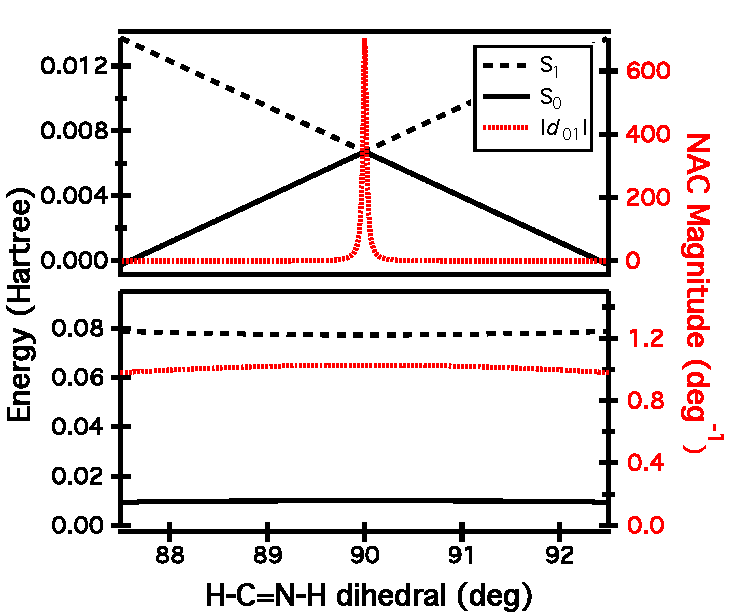
\includegraphics[width=\textwidth]{gs_es_dercp} 
  \caption{ }
  \label{fig:gs_es_dercp}
  \end{subfigure}
  \begin{subfigure}[b]{0.40\textwidth}
  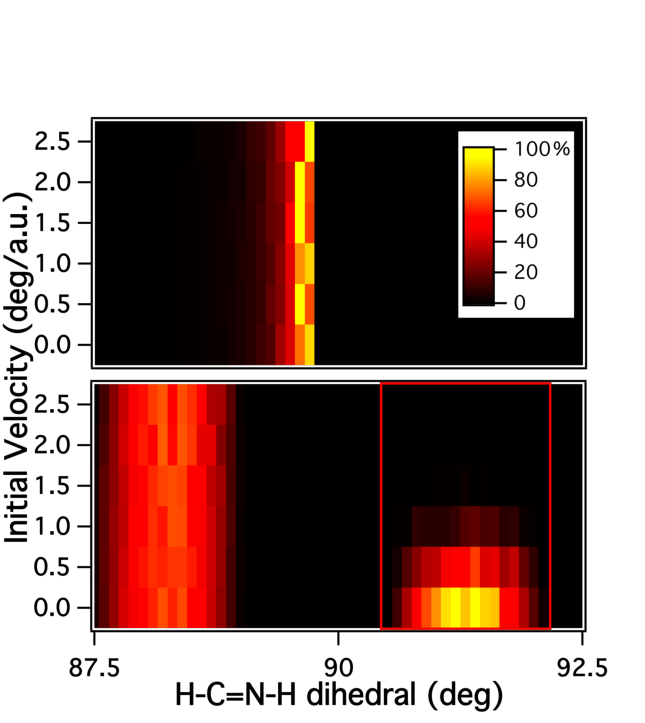
\includegraphics[width=\textwidth]{stacked_hops} 
  \caption{ }
  \label{fig:hops}
  \end{subfigure}
  \caption{\footnotesize (a) Potential energy surfaces for ground and excited
  states, and the coupling strength between the two states with respect to the
  dihedral angle in the vicinity of the minimum energy crossing point between
  S$_0$ and S$_1$ from the pp-TDA (top frame) and CIS (bottom frame) approaches.
  (b) Color maps showing the distribution of configurations at which hops from
  S$_1$ to S$_0$ occur for the different initial velocities resolved at the
  pp-TDA (top frame) and CIS (bottom frame) levels of theory (area in red box
  magnified, after normalization, 1000$\times$ for visibility.)}
\end{figure}

To demonstrate the performance of the pp-TDA within TSH over single reference
methods such as configuration interaction singles (CIS), we simulated the ground
state recovery dynamics for a small iminium ion, H$_2$C=NH$_2^+$, known to
readily photo-isomerize via a conical-intersection-mediated, non-radiative decay
from S$_1$ to the ground state, S$_0$, using both the CIS and pp-TDA description
of the adiabats. The important difference between the two methods is in an
asymmetric treatment of electron correlation in the ground and excited states in
the CIS, while the pp-TDA treats all of the states on the same footing. To
ensure that our TSH simulation transversed the conical intersection, we
restricted the nuclear trajectories to the well--established isomerization
coordinate of the dihedral rotation.  Potential energy surfaces and NAC 
strengths along the reaction coordinate are collected in \cref{fig:gs_es_dercp}. 
%There are several conditions for determining the presence of a conical
%intersection of PESs. A necessary and sufficient condition is the presence of a
%degeneracy as well as a spike in the NAC magnitude in the neighborhood of the
%proposed conical intersection (technically the NAC becomes undefined at the
%conical intersection which exists at exactly one point on the PES).
It is clear that the conical intersection along the isomerization coordinate is
not captured in the CIS PES, while the pp-TDA exhibits the correct behavior.

10$^6$ TSH trajectories for a series of 6 initial velocities were considered for
each of the two electronic structure methods.  In all cases the electronic
superposition was initialized as a pure (S$_1$) state, and the dihedral angle
was chosen to be 87.5 degrees so that the dynamics are started in the upper
state near to the region of strongest coupling. Relation profiles for the S$_1$
to S$_0$ inter-conversion are given in the form of a heat plot in
\cref{fig:hops}. There are two characteristics of dynamics in the neighborhood
of conical intersections and are of interest in the relaxation
profiles\cite{Hynes14_97}. First of which is internal conversion from S$_1$
$\rightarrow$ S$_0$ should be localized near the conical intersection. This
feature is clearly captured by the pp-TDA, while CIS suffers a broad relaxation
profile that is qualitatively incorrect. 
%This incorrect profile is due to the artificially early onset of the
%NAC along the isomerization coordinate which is a result of improper description
%of the conical intersection.
The second feature is that all of the classical nuclear trajectories should
interconvert before the conical intersection. This feature is captured in the
pp-TDA, even in the initial velocity limit. In the CIS simulation, a small
portion of the trajectories hop at configuration past the conical intersection
at the low initial velocity limit. This means that those trajectories
transversed the conical intersection throughout the simulation. This
qualitatively incorrect behavior would lead to uncharacteristically long
relaxation rates over the pp-TDA.

Although the pp-TDA has been shown to perform quite well in the proper treatment
of excited to ground state interconversion, its use as a general tool is quite
limited due to the presence of instabilities in the underlying reference
determinant throughout the dynamics simulation. 
%The reason for this is the fact
%that the reference determinant one that is optimized with respect to the ($N-2$)
%cation of the molecular system. In the case of the iminum ion, the ground state
%geometry is planar, while the conical intersection is located at the point where
%diheral of the two functional groups is at 90 degrees. 
In the case of the
$N$-electron system, the ground state HF wave function is perfectly stable at
the ground state, while there exists a triplet instability in the singlet HF
wave function at the conical intersection. Interestingly, the exact opposite
problem occurs in the ($N-2$) electron system. This indicates a fundamental
problem in the single Slater determinantal wave function description of
molecular systems. One of the base assumptions of post SCF methods in electronic
structure is that the underlying reference determinant is stable at a given
molecular geometry. If that assumption is no longer valid, the behavior of
these methods often become ill defined. Thus it is important to utilize methods
that will ensure variational stability throughout the entire nuclear
configuration space, such as more general CAS methods.


\linespread{1.0}
\section{Relativistic Non--Adiabatic Molecular Dynamics with CI Wave Functions}
\linespread{1.5}
\label{sec:Future}

Extension of existing methodologies using relativistic CI wave functions for use
in non--adiabatic dynamics is a challenging endeavor. Existing relativistic
treatments of CI wave function have been limited to single--point calculations,
and many of the ingredients needed for use with molecular dynamics have not yet
been developed.
{\bf As most of the computational machinery required to extend trajectory
surface hopping to relativistic CI wave functions, the majority of the proposed
research will be focused on developing the methods required to facilitate the
extension.}

Examining \cref{eq:EOMCs,eq:HamiltonianElec,eq:NAC,eq:Newton}, it is clear to
see that if one has access to geometric gradients ($\nabla E_c$) and NAC tensor
elements, one can perform TSH using that method, neither of which are readily
available for relativistic CI wave functions. As for the geometric gradients,
some methods have been proposed for other, more complicated relativistic
two--component methods\cite{Nakai16_JCTC2181,Cremer15_JCP214106} than the X2C
Hamiltonian in the mean--field description of the wave function, but the current
state of geometric gradients for the X2C is limited to scalar relativistic
treatment which neglect SOC\cite{Gauss11_JCP084114}. No attempts have been made
to evaluate geometric gradients in the two--component relativistic treatment of
CI wave functions. Although gradients and NAC tensor elements for
non--relativistic CI wave functions have existed for many years, extension to
two--component relativistic methods is non--trivial as they both involve
differentiation of the transformation operator, $\op{U}$.

In the X2C treatment of CI wave functions, the expressions for the energy
gradients and NAC tensor elements look nearly identical. The only differences
between them are scaling of certain terms by energy differences, which are
inconsequential to the difficulties of the X2C method. Here, I will only discuss
the energy gradient, keeping in mind that a virtually identical procedure holds
for the NAC tensor elements. The energy expression for the CI eave function is
given by,
\begin{align}
&\mathcal{E}_I = h^\mathrm{X2C}_{pq}\gamma^I_{pq} + 
 (pq|rs) \Gamma^I_{pqrs} \\
&\gamma^I_{pq} = 
  \sum_{\alpha,\beta \in \mathcal{K}} 
  \innerop{\psi_\alpha}{a_p^\dagger a_q}{\psi_\beta} d_\alpha^{I*} d_\beta^I
  \qquad
  \Gamma^I_{pqrs} = \frac{1}{2} \sum_{\alpha,\beta\in\mathcal{K}}
  \innerop{\psi_\alpha}{a_p^\dagger a_q a_r^\dagger a_s - \delta_{qr}a_p^\dagger
  a_s}{\psi_\beta} d_\alpha^{I*} d_\beta^I
\end{align}
Here, the time and parameter dependence has been dropped for brevity. The term
of consequence is in $\vc{h}^\mathrm{X2C}$, which is the large component part of
the two--component transformed one--electron Dirac Hamiltonian in the MO basis.
As the energy is variational with respect to the expansion coefficients, the
energy gradient only involves derivatives of the Hamiltonian
\begin{align}
&\nabla_\xi \mathcal{E}_I = \left(\nabla_\xi h^\mathrm{X2C}_{pq}\right)
  \gamma^I_{pq} + 
 \left( \nabla_\xi (pq|rs) \right)\Gamma^I_{pqrs} \quad.
\end{align}
The derivative of the X2C core Hamiltonain may be written as
\begin{equation}
\nabla_\xi h^\mathrm{X2C}_{pq} = \nabla_\xi\int_{\mathbb{R}^3} \phi_p(\vc{r})
  \mathcal{H}_+ \phi_q(\vc{r}) \text{
 }\mathrm{d}^3\vc{r} \quad,
\end{equation}
which involves derivatives of $\mathcal{H}_+$. Recalling the form of the
two--component transformation, the derivatives of $\mathcal{H}_+$ are dependant
on derivatives of $\mathcal{U}$,
\begin{equation}
\begin{pmatrix} \nabla_\xi \mathcal{H}_+ && 0_2 \\ 0_2 && \nabla_\xi
\mathcal{H}_- \end{pmatrix} =
2\mathcal{U}^\dagger\mathcal{H}_D\left(\nabla_\xi\mathcal{U}\right) +
\mathcal{U}^\dagger \bpar{\nabla_\xi\mathcal{H}_D} \mathcal{U}\quad.
\end{equation}
While the gradients of the Dirac Hamiltonian have been known for some time, the
gradients of $\mathcal{U}$ are dependant on the two--componant transformation
scheme. In general, the form of the derivative of $\mathcal{U}$ is non--trival
due to the fact that it is typically obtained via an eigendecomposition. There
exist schemes to perform these types of differentiations analytically, however
they have now yet been extension to the X2C method with the inclusion of SOC.
Once the deivatives of $\mathcal{U}$ are obtained, assembly of the geometric
derivatives and NAC tensor elements is possible. {\bf Thus, one of the primary
tasks in the proposed research is to facilitate the efficient evaluation 
gradient and non--adiabatic coupling tensor elements for X2C CI wave functions.}

Once TSH may be performed using X2C CI wave functions, there exist many possible
test cases to validate the accuracy and usefulness of the method. Currently, my
plan is to choose a relatively small, one-dimensional test case much analogous
to the one presented in \cref{sec:pp-TSH}. This condition is nicely met with the
photodissociation of HCo(CO)$_4$. It is well known that a key mehanistic point
of the photodissociation of  HCo(CO)$_4$ involves a rapid ($<$50ps) ISC process
from the first singlet to first triplet excited state. This system has already
been studied using a perturbative treatment of SOC in CAS wave functions by
Daniel \emph{et al.} In their study, they discovered that the ISC in this
process may be modelled along a single one--dimension reaction coordinate. 
{\bf To validate this method, I will attempt to recreate and improve upon
existing studies of the photodissociation of HCo(CO)$_4$. Such a study will
allow me to asses the accuracy and usefulness of trajectory surface hopping
using relativistic CI wave functions.}

I beleive that the \emph{ab initio} treatment of SOC throughout a TSH simulation
will provide a marked improvement over the perturbative treatments that
currently exist in the literature. Futher, as previous studies have been limited
to model reaction coordinates, such a direct relativistic treatment of SOC will
provide a much needed generalization to current methodologies. As my proposed
treatment makes minimal assumptions about the underlything quantum mechanics of
the molecular system, it may be used as a general tool to solve current and
future problems in the field of realtivistic non--adiabatic dyanamics.



\linespread{1.0}
\bibliography{Journal_Short_Name,ppSH,Li_Group_References,GE,DBWY,Egidi_References}
\end{document}
